% !TeX root = ../main.tex
% -*- coding: utf-8 -*-
% !TeX root = ../main.tex
% -*- coding: utf-8 -*-

\chapter{基于模拟采样的强化学习算法}

基于 Markov 性质的前提,即在 Markov 决策过程中,之前给出的基于迭代求解 Bellman 方程的强化学习算法非常简洁清晰,但该算法对环境条件的依赖性较强,同时还需要显示地知道环境的动态分布 $p(s',r|s,a)$ ,对于传统的“完全信息博弈”而言这一点非常容易满足,但对于实际中更常见且更复杂的“不完全信息博弈”,我们并不能准确得知 $p(s',r|s,a)$ ,传统的强化学习算法很难克服这一问题\cite{sutton2018reinforcement},所以需要在其基础上做进一步改进,通过模拟采样的方法来获取和近似估计回报值,避免对环境进行模型重建。

\section{Monte Carlo 模拟}

Monte Carlo 方法\cite{goodfellow2016deep}\cite{robert2013monte}也称统计模拟方法,上一章的基于解 Bellman 方程的强化学习算法,由于依赖环境动态信息 $p(s',r|s,a)$ ,在不完全信息下无法得到此式,仅适合处理传统的完全信息问题,但借由 Monte Carlo 模拟方法,可以通过模拟和采样来近似地获得环境信息,进而也能使用强化学习来解决不完全信息问题。

在未知 $p(s',r|a,s)$ 的情况下,算法不能使用的根本原因在于无法计算 Bellman 方程 \ref{eq:bellmaneq} 中的 $\sum_{s',r}p(s',r|s,a)[r+\gamma v(s')]$ ,即无法清晰地预知未来的状态与反馈信息,其核心在于每一步的奖励值 $r$ 无法取得,而如果采用 Monte Carlo 方法进行模拟,可以进行大量模拟实验,通过计算样本回报值的均值,便能有效解决这一点。

记某个回合中通过模拟得到的反馈数据序列为 $\left\{R_0, R_1, R_2, \ldots, R_T\right\}$ ,在这一回合中,可计算出时刻 $t$ 对应的回报值

\begin{equation}
    G_t = R_{t+1} + \gamma R_{t+2} + \gamma^2 R_{t+3} + \cdots + \gamma^{T-t-1} R_T
\end{equation}

计算 Monte Carlo 模拟获得的回报值均值,可以作为价值函数的估计,即可得到基于 Monte Carlo 模拟的强化学习算法:

\begin{algorithm}[H]
    \caption{基于 Monte Carlo 模拟的强化学习算法}
    \begin{algorithmic}[1] %每行显示行号
        \State 将 $\pi$ 初始化为一个随机策略
        \State 初始化向量 $Q(s,a), \forall s\in \mathcal S,a\in \mathcal{A}(s)$
        \State 将 $Returns(s,a)$ 初始化为一个空数组,$\forall s\in\mathcal S,a\in\mathcal{A}(s)$
        \Loop
        \State 随机选取初始状态 $S_0\in\mathcal S$ 和初始行动 $A_0\in\mathcal{A}(S_0)$
        \State 服从现有策略 $\pi$ 与环境交互生成一个回合片段
        \State 得到 $S_{0}, A_{0}, R_{1}, S_{1}, A_{1}, R_{2}, \ldots, S_{T-1}, A_{T-1}, R_{T}$
        \State $G\leftarrow 0$
        \For{回合中的每一步 $t=T-1, T-2, \ldots, 0$, }
        \State $G \leftarrow \gamma G+R_{t+1}$
        \If{$S_t,A_t$ 在 $S_{0}, A_{0}, S_{1}, A_{1} \ldots, S_{t-1}, A_{t-1}$ 中出现过}
        \State 将 $G$ 追加进数组 $Returns(S_t,A_t)$
        \State $Q(S_t,A_t)\leftarrow \mathrm{average}(Returns(S_t,A_t))$
        \State $\pi(S_t)\leftarrow \arg\max_aQ(S_t,a)$
        \State 跳出本层循环
        \EndIf
        \EndFor
        \EndLoop
        \State
        \State 输出最终策略 $\pi$
    \end{algorithmic}
\end{algorithm}

\section{Bootstrap 自助学习}

Monte Carlo 算法的价值函数更新式为

\begin{equation}\label{eq:mcupdate}
    V(S_t)\leftarrow V(S_t)+\alpha\left[G_t-V(S_t)\right]
\end{equation}

在 Monte Carlo 算法中,由于需要等待一个完整的片段结束,得到每个时间点的奖励值 $R_t$,才能返回到之前各时间点求得对应的回报值 $G_t = R_{t+1}+\gamma R_{t+2}+\gamma^2 R_{t+3}+\cdots+\gamma^{T-t-1} R_T$ 。这一缺点限制了算法的使用场景,其高延迟使得算法无法处理实时学习问题,而 Monte Carlo 本身需要等待一个完整回合结束的特点也导致无法处理连续型问题。

为了能够做到实时更新,即需要在每个时间点 $t$ 得到当前反馈奖励值 $R_t$ 时能够即使更新,而非累积足够多反馈奖励值才去更新,故考虑结合统计学中的 Bootstrap 思想\cite{efron1994introduction}\cite{2014wzjstatistics},利用“重抽样”的思想来尽可能利用信息价值,根据当前时刻 $t$ 下的信息进行一定程度的“再利用”,使用估计值来替换 $G_t$ 。

具体地,记 $\widehat{V}(S_{t})$ 表示 $V({S_t})$ 的一个估计值,则有

\begin{equation}\label{eq:vhat}
    \widehat{V}(S_{t+1}) \approx R_{t+2} + \gamma R_{t+3} + \gamma^2 R_{t+4} + \cdots
\end{equation}

从而可得到

\begin{equation}\label{eq:toreplacegt}
    \begin{aligned}
        G_t &= R_{t+1}+\gamma R_{t+2}+\gamma^2 R_{t+3}+\gamma^3 R_{t+4}+\cdots\\
        &=R_{t+1}+\gamma\left[R_{t+2}+\gamma R_{t+3}+\gamma^2 R_{t+4}+\cdots\right]
    \end{aligned}
\end{equation}

将\ref{eq:vhat}代入\ref{eq:toreplacegt}可得

\begin{equation}\label{eq:replacedgt}
    G_t \approx R_{t+1} +\gamma \widehat{V}(S_{t+1})
\end{equation}

将\ref{eq:replacedgt}式代入更新式\ref{eq:mcupdate}中,可得到改进后的更新式

\begin{equation}\label{eq:tdupdate}
    V(S_t)\leftarrow V(S_t)+\alpha\left[R_{t+1}+\gamma \widehat{V}(S_{t+1})-V(S_t)\right]
\end{equation}

由于上述更新式使用前后两个时刻的 Bootstrap 估计值之差来作为更新量,故称使用上述更新式来学习价值函数的方法为{\jiacu 时序差分学习}。显然可见,时序差分学习可以在每一时间点 $t$ 进行更新和学习,无需等待完整的片段结束得到 $G_t$ 才去更新,其效率要比普通的 Monte Carlo 方法更高,且因此特性而适用于连续型的非片段问题。

\subsection{Q-Learning 算法}

将时序差分算法更新式\ref{eq:tdupdate}中的状态价值函数 $V(s)$ 改为行动价值函数 $Q(s,a)$ ,写作

\begin{equation}
    Q(S_t,A_t)\leftarrow Q(S_t,A_t)+\alpha\left[R_{t+1}+\gamma \widehat{Q}(S_{t+1},A_{t+1})-Q(S_t,A_t)\right]
\end{equation}

在强化学习的实际应用中,需要为行动价值函数 $\widehat{Q}(S_t,A_t)$ 指定一个具体的估计值。由于在更新过程中,后一次行动的决策更倾向于选择前一次价值 $Q$ 更大的行动,因此最直观的考虑是选取 $\max_a Q_{old}(S_t,a)$ 作为 $Q_{new}(S_t,A_t)$ 的 Bootstrap 估计值,此时的算法更新式为

\begin{equation}\label{eq:qlearning}
    Q(S_t,A_t)\leftarrow Q(S_t,A_t)+\alpha\left[R_{t+1}+\gamma  \max\limits_aQ(S_{t+1},a)-Q(S_t,A_t)\right]
\end{equation}

由于该算法以行动价值函数 $Q(s,a)$ 为核心,基于这一评估指标进行各种决策学习,故称使用了该更新式的强化学习算法为{\jiacu\ Q-Learning 算法}。Q-Learning 算法的详细流程如下:

\begin{algorithm}[H]
    \caption{Q-Learning 算法}
    \begin{algorithmic}[1] %每行显示行号
        \State 将 $\pi$ 初始化为一个随机策略
        \State 初始化向量 $Q(s,a), \forall s\in \mathcal S,a\in \mathcal{A}(s)$
        \Loop
        \State 随机选取初始状态,记作 $S$
        \Repeat
        \State 根据价值函数 $Q$ 选取状态 $S$ 下的最优行动 $A$
        \State 采取行动 $A$ ,观测环境反馈 $R$ 以及后续状态 $S'$
        \State $Q(S,A)\leftarrow Q(S,A)+\alpha\left[R+\gamma  \max\limits_aQ(S',a)-Q(S,A)\right]$
        \State $S\leftarrow S'$
        \Until{$S$ 为终止状态}
        \EndLoop
        \State
        \State 根据学得的 $Q$ 函数决定并输出最终策略 $\pi$
    \end{algorithmic}
\end{algorithm}

\subsection{$\varepsilon$-贪心 Q-Learning 算法}

在前面的算法中,我们在得到价值函数之后,都是直接对其取 $\arg\max$ 来作为最优策略,这是完全的贪心学习\cite{edmonds1971matroids},初期如果过于贪心去信赖尚不完善的价值函数,容易导致策略收敛在局部最优值,所以需要将贪心的程度适当降低,于是提出下面的 $\varepsilon$-贪心学习算法

\begin{Definition}
    在强化学习中,若决策者以 $1-\varepsilon(0<\varepsilon<1)$ 的概率采取贪心行动,以 $\varepsilon$ 的概率随机选择一个行动 $a$ ,称这样的学习方法为 $\varepsilon$-贪心学习算法。
\end{Definition}

在强化学习中,当决策者采取 $\varepsilon$ 的概率随机采取行动而非贪心选择当前价值最大的行动时,认为这是在{\jiacu 探索},反之则是在{\jiacu 利用}。适当地进行探索,可以加速对环境未知信息的学习,同时也有利于及时跳出局部最优点,同时,只要 $\varepsilon$ 不设太大,以 $1-\varepsilon$ 的概率来利用已学习的知识,在其所在时刻下相比纯贪心学习也几乎不会有损失,能够兼顾信息探索率和信息的充分利用率。

具体地,给出贪心学习下的策略函数定义

\begin{Definition}
    设
    \begin{equation}
        \pi(a|s)=
        \begin{cases}
            \frac{\varepsilon}{|\mathcal A(s)|}&, a\text{为非贪心行动}\\
            1-\varepsilon-\frac{\varepsilon}{|\mathcal A(s)|}&, a\text{为贪心行动}
        \end{cases}
    \end{equation}

其中 $|\mathcal{A}(s)|$ 表示行动空间 $\mathcal{A}(s)$ 中的元素个数。称这样的策略 $\pi$ 是 $\varepsilon$-贪心策略。
\end{Definition}

下面证明,将非贪心行动的概率逐渐降低、贪心行动的概率逐渐提高,能够提高期望价值函数。

\begin{proof}
    记 $\pi'$ 为贪心改进后的策略,其表达式为
    \begin{equation}
        \pi'(a|s)=
        \begin{cases}
            \frac{\varepsilon}{|\mathcal A(s)|}&, a\text{为非贪心行动}\\
            1-\varepsilon-\frac{\varepsilon}{|\mathcal A(s)|}&, a\text{为贪心行动}
        \end{cases}
    \end{equation}
    而改进前的策略为
    \begin{equation}
        \pi(a_i|s)=
\begin{cases}
\frac{\varepsilon}{|\mathcal A(s)|}+\delta_i&,a_i\neq a_*\\
1-\frac{(|\mathcal A(s)|-1)\varepsilon}{|\mathcal A(s)|}-\sum_{a_i\neq a_*}\delta_i&,a_i=a_*
\end{cases}
    \end{equation}
    其中 $\delta_i>0$,表示策略改进的差异量,则有
    \begin{equation}\label{eq:beforeineq}
        \begin{aligned}
            v_{\pi'}(s)&=\sum_a
            \pi'(a|s)q_\pi(s,a)\\
            &=\frac{\varepsilon}{|\mathcal A(s)|}\sum_aq_\pi(s,a)+(1-\varepsilon)\max\limits_aq_\pi(s,a)
            \end{aligned}
    \end{equation}
    记 $M=\max\limits_aq_\pi(s,a)$ ,首先证明不等式
    \begin{equation}\label{eq:ineq1}
        \displaystyle \max\limits_aq_\pi(s,a)\geq\sum_a\frac{\pi(a|s)-\frac{\varepsilon}{|\mathcal A(s)|}}{1-\varepsilon}q_\pi(s,a)
    \end{equation}
    该不等式证明如下:
    \[
        \begin{aligned}
            &\sum_a\frac{\pi(a|s)-\frac{\varepsilon}{|\mathcal A(s)|}}{1-\varepsilon}q_\pi(s,a)\\
            &=\frac{\pi(a_*|s)-\frac{\varepsilon}{|\mathcal A(s)|}}{1-\varepsilon}M+\sum_{a_i\neq a_*}\frac{\pi(a_i|s)-\frac{\varepsilon}{|\mathcal A(s)|}}{1-\varepsilon}q_\pi(s,a_i)\\
            &= \frac{1-\frac{(|\mathcal A(s)|-1)\varepsilon}{|\mathcal A(s)|}-\sum_{a_i\neq a_*}\delta_i-\frac{\varepsilon}{|\mathcal A(s)|}}{1-\varepsilon}M+\sum_{a_i\neq a_*}\frac{\delta_i}{1-\varepsilon}q_\pi(s,a_i)\\
            &=\frac{1-\varepsilon}{1-\varepsilon}M-\frac{1}{1-\varepsilon}\sum_{a_i\neq a_*}\delta_iM+\frac{1}{1-\varepsilon}\sum_{a_i\neq a_*}\delta_iq_\pi(s,a_i)\\
            &=M-\frac{\sum_{a_i\neq a_*}\delta_i}{1-\varepsilon}(M-q_\pi(s,a_i))\\
            &\leq M=\max\limits_aq_\pi(s,a)
            \end{aligned}
    \]
    不等式\ref{eq:ineq1}得证,将其代回\ref{eq:beforeineq}中,则有
    \[
        \begin{aligned}
            v_{\pi'}(s)&\geq\frac{\varepsilon}{|\mathcal A(s)|}\sum_aq_\pi(s,a)+(1-\varepsilon)\sum_a\frac{\pi(a|s)-\frac{\varepsilon}{|\mathcal A(s)|}}{1-\varepsilon}q_\pi(s,a)\\
            &=\frac{\varepsilon}{|\mathcal A(s)|}\sum_aq_\pi(s,a)-\frac{\varepsilon}{|\mathcal A(s)|}\sum_aq_\pi(s,a)+\sum_a\pi(a|s)q_\pi(s,a)\\
            &=v_\pi(s)
            \end{aligned}
    \]
    证毕。
\end{proof}

因此证得,将非贪心行动的概率逐渐降低、贪心行动的概率逐渐提高,能够提高期望价值函数,从而若将$\varepsilon$-贪心策略与 Q-Learning 算法结合,由于$\varepsilon$-贪心策略有着较好的跳出局部最优点的性质,且因 Q-Learning 算法下期望价值函数的逐渐提高能够确保算法的收敛性,便能做到既提升算法跳出局部最优点的鲁棒性,同时也促进算法的收敛性。两种方法相结合后的算法流程如下:

\begin{algorithm}[H]
    \caption{基于 Q-Learning 的 $\varepsilon$-贪心强化学习算法}
    \begin{algorithmic}[1] %每行显示行号
        \State 将 $\pi$ 初始化为一个随机策略
        \State 初始化向量 $Q(s,a), \forall s\in \mathcal S,a\in \mathcal{A}(s)$
        \Loop
        \State 随机选取初始状态,记作 $S$
        \Repeat
        \State 在 $S$ 状态下,根据策略 $\pi$ 选择最优行动 $A$
        \State 采取行动 $A$ ,观测环境反馈 $R$ 以及后续状态 $S'$
        \State $Q(S,A)\leftarrow Q(S,A)+\alpha\left[R+\gamma  \max\limits_aQ(S',a)-Q(S,A)\right]$
        \State $A^*\leftarrow\arg\max_aQ(S_t,a)$
        \For{$\forall a\in\mathcal{A}(S)$}
        \If{$a\neq A^*$}
        \State $\pi(a|s)\leftarrow \frac{\varepsilon}{|\mathcal A(s)|}$
        \Else
        \State $\pi(a|s)\leftarrow 1-\varepsilon-\frac{\varepsilon}{|\mathcal A(s)|}$
        \EndIf
        \EndFor
        \State $S\leftarrow S'$
        \Until{$S$ 为终止状态}
        \EndLoop
        \State
        \State 输出最终策略 $\pi$
    \end{algorithmic}
\end{algorithm}

\chapter{基于 Q-Learning 的机器学习方法}

在 Q-Learning 算法中,主要目的是通过更新式 \ref{eq:qlearning} 来逼近最优行动值函数 $Q^*(s,a)$ 。具体地,在每一步中用新的估计值 $r+\gamma \max_aQ(s,a)$ 来逼近 $Q(s,a)$ ,注意到,$Q$ 函数的参数 $s\in\mathcal S, a\in\mathcal A$ 所在的参数空间都很大,对参数进行逐个更新的效率很低,使得该算法实用性并不高。为了提高算法效率,提升算法的实用性,应当将函数参数化后,使用机器学习方法进行更新和训练,结合深度神经网络来训练 $Q$ 函数。

\section{梯度下降 Q-Learning 算法}

首先将价值函数 $Q$ 参数化,设其参数为 $\boldsymbol{w}$ ,记参数化的价值函数为 $\widehat{Q}(s,a,\boldsymbol{w})$。为了使参数化的价值函数 $\widehat{Q}$ 能逼近真实价值函数 $Q$ ,仍以 Q-Learning 算法的更新公式为核心,在其基础上使用梯度下降法\cite{tsitsiklis1997analysis}\cite{bottou2010large}\cite{sutton2009fast}。

在 Q-Learning 梯度下降法中,以更新前后的行动价值函数均方误差为损失函数,定义为

\begin{equation}
    J(\boldsymbol{w}) = \frac{1}{2}\left[R_{t+1}+\gamma\max_a\widehat{Q}(S_{t+1},a,\boldsymbol{w})-\widehat{Q}(S_t,A_t,\boldsymbol{w})\right]^2
\end{equation}

根据梯度下降法,以优化降低损失函数 $J(\boldsymbol{w})$ 为目标进行更新,其更新式为

\begin{equation}\label{eq:qlearninggrad}
\begin{aligned} \boldsymbol{w}_{t+1} =&\boldsymbol{w}_{t}-\alpha\nabla J(\boldsymbol{w}) \\ =&\boldsymbol{w}_{t}+\alpha\left[R_{t+1} - \gamma \max _{a} \widehat{Q}\left(S_{t+1}, a, \boldsymbol{w}_{t}\right)-\widehat{Q}\left(S_{t}, A_{t}, \boldsymbol{w}_{t}\right)\right]\\&\times\left[\gamma\nabla \max _{a} \widehat{Q}\left(S_{t+1}, a, \boldsymbol{w}_{t}\right)-\nabla \widehat{Q}\left(S_{t}, A_{t}, \boldsymbol{w}_{t}\right)\right] \end{aligned}
\end{equation}

其中,$\alpha$ 是梯度下降法中的更新速率,用来控制梯度更新的速度。最终更新停止后得到的 $\boldsymbol{w}^*$ 即可用以还原出参数化的价值函数 $\widehat{Q}^*(s,a,\boldsymbol{w}^*)$ ,进而可以给出决策函数 $\pi$ 。可将 $\varepsilon$-贪心学习与梯度下降 Q-Learning 算法相结合,详细的算法流程如下:

\begin{algorithm}[H]
    \caption{$\varepsilon$-贪心梯度下降 Q-Learning 算法}
    \begin{algorithmic}[1] %每行显示行号
        \State 将 $\pi$ 初始化为一个随机策略
        \State 初始化参数函数 $\widehat{Q} : \mathcal{S} \times \mathcal{A} \times \mathbb{R}^{d} \rightarrow \mathbb{R}$
        \State 设定超参数:步长 $\alpha>0$,贪心率 $\varepsilon>0$
        \State 将价值函数的权重 $\boldsymbol{w}\in\mathbb{R}^d$ 初始化
        \Loop
        \State 随机选取初始状态,记作 $S$
        \Repeat
        \State 在 $S$ 状态下,根据策略 $\pi$ 选择最优行动 $A$
        \State 采取行动 $A$ ,观测环境反馈 $R$ 以及后续状态 $S'$
        \If {$S'$ 不是终止状态}
        \State $\nabla\boldsymbol{J}\leftarrow \gamma\nabla\max_a\widehat{Q}(S',a,\boldsymbol{w})-\nabla\widehat{Q}(S,A,\boldsymbol{w})$
        \State $\boldsymbol{w}\leftarrow\boldsymbol{w} - \alpha\left[R+\gamma\max_a\widehat{Q}(S',a,\boldsymbol{w})-\widehat{Q}(S,A,\boldsymbol{w})\right]\nabla\boldsymbol{J}$
        \Else
        \State $\nabla\boldsymbol{J}\leftarrow -\nabla\widehat{Q}(S,A,\boldsymbol{w})$
        \State $\boldsymbol{w}\leftarrow\boldsymbol{w} - \alpha\left[R-\widehat{Q}(S,A,\boldsymbol{w})\right]\nabla\boldsymbol{J}$
        \EndIf
        \State $A^*\leftarrow\arg\max_aQ(S_t,a)$
        \For{$\forall a\in\mathcal{A}(S)$}
        \If{$a\neq A^*$}
        \State $\pi(a|s)\leftarrow \frac{\varepsilon}{|\mathcal A(s)|}$
        \Else
        \State $\pi(a|s)\leftarrow 1-\varepsilon-\frac{\varepsilon}{|\mathcal A(s)|}$
        \EndIf
        \EndFor
        \State $S\leftarrow S'$
        \Until{$S$ 为终止状态}
        \EndLoop
        \State
        \State 输出最终策略 $\pi$
    \end{algorithmic}
\end{algorithm}

\section{自适应 Deep Q-Learning 算法}

上一节已将 Q-Learning 算法与机器学习中的梯度下降算法相结合,在此基础上,可以通过建立神经网络来实现算法的梯度更新部分\cite{hecht1992theory},便能进一步提高行动价值函数 $\widehat{Q}$ 的收敛速度。

\begin{figure}[H]
    \centering
    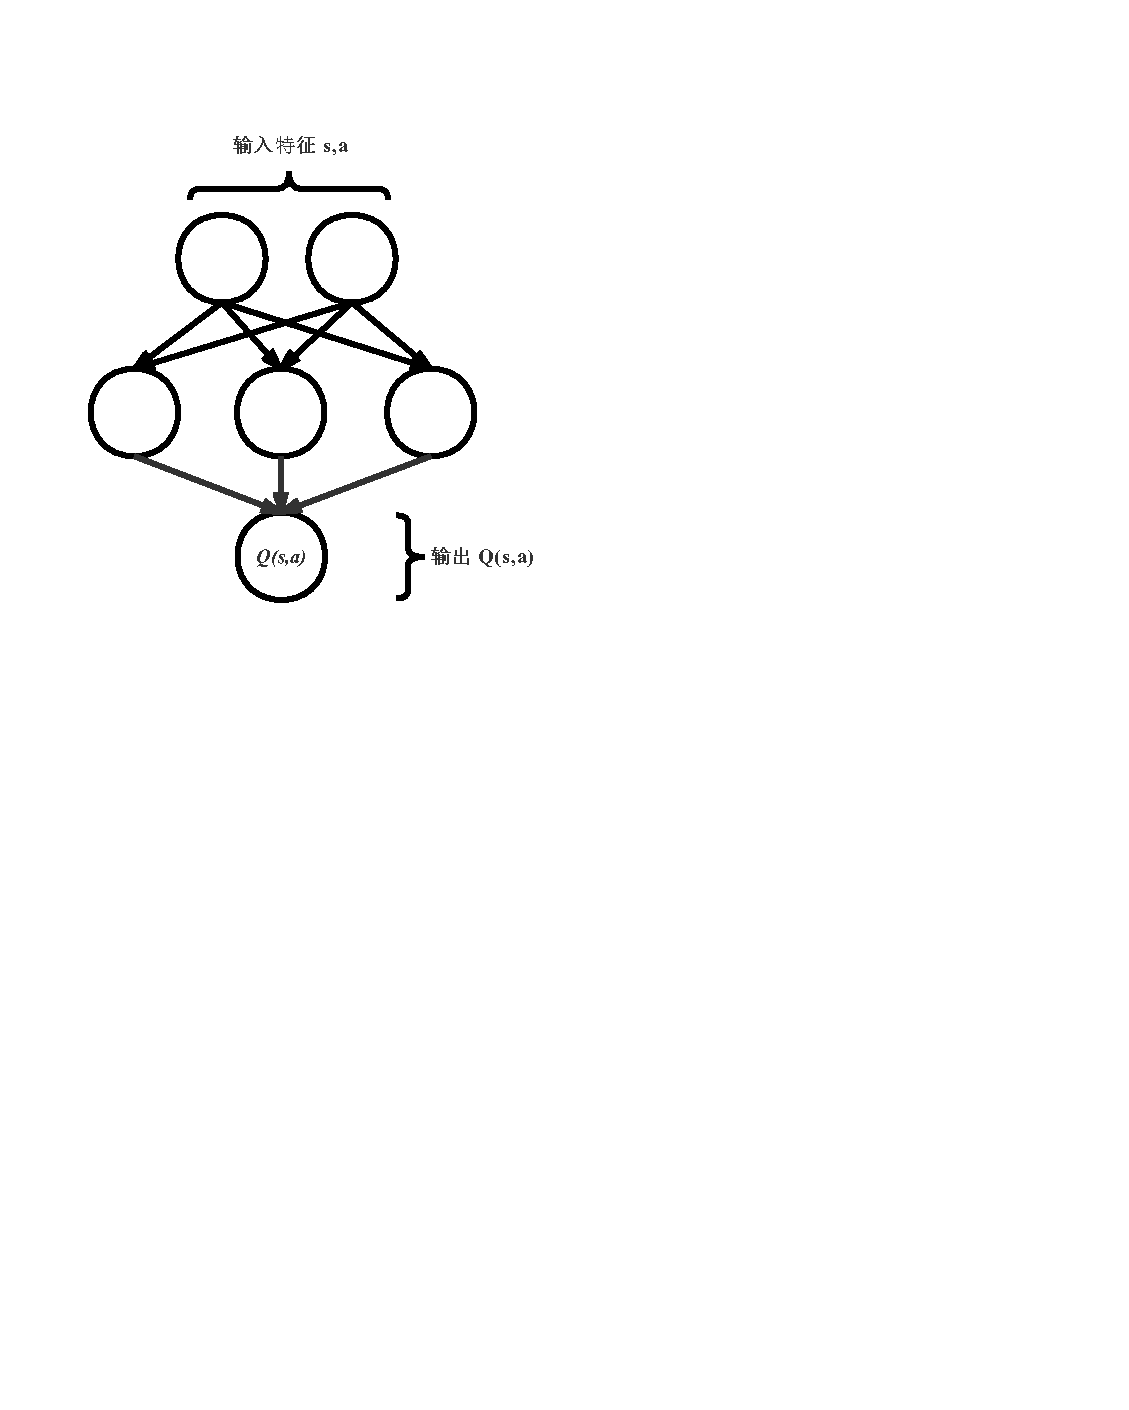
\includegraphics[width=0.5\textwidth]{DQN-show.pdf}
    \caption{Deep Q-Network 示意图}
\end{figure}

如上图所示,将实时数据流中的状态和行动作为特征向量传入神经网络的输入层,基于参数化的 Q-Learning 公式

\begin{equation}
\begin{aligned} \boldsymbol{w}_{t+1} =&\boldsymbol{w}_{t}-\alpha\nabla J(\boldsymbol{w}) \\ =&\boldsymbol{w}_{t}+\alpha\left[R_{t+1} - \gamma \max _{a} \widehat{Q}\left(S_{t+1}, a, \boldsymbol{w}_{t}\right)-\widehat{Q}\left(S_{t}, A_{t}, \boldsymbol{w}_{t}\right)\right]\\&\times\left[\gamma\nabla \max _{a} \widehat{Q}\left(S_{t+1}, a, \boldsymbol{w}_{t}\right)-\nabla \widehat{Q}\left(S_{t}, A_{t}, \boldsymbol{w}_{t}\right)\right] \end{aligned}
\end{equation}

通过神经网络的反向梯度传递来更新权值参数,进而实现梯度下降算法\cite{hecht1992theory}。称使用深度神经网络进行梯度下降的 Q-Learning 算法为 Deep Q-Learning 算法,将该神经网络结构称为 Deep Q-Network 。

在实际的应用场景中,不完全信息博弈常为多人对战类游戏,因此需要针对性地优化前面所描述的 Q-Learning 算法。

在 Q-Learning 中,基于 Bootstrap 思想,采用了 $\max_aQ(s,a)$ 作为 $Q(s,a)$ 的更新估计值,但在神经网络中大量使用 $\max$ 函数会带来一定的偏差值,带来决策误差。为了解决这一问题,需要使用两个神经网络交替使用来抵消这一偏差值。

\begin{Theorem}\label{the:doubledqn}
    记两个独立的 Deep Q-Network 分别为 $Q_1,Q_2$ ,并假定他们能无偏估计真实值,即满足条件 $\mathbb{E}\left[Q_1(s,a)\right] = q(s,a)$,$\mathbb{E}\left[Q_2(s,a)\right] = q(s,a)$ 。若使用 $Q_1$ 来参与行为决策,使用 $Q_2$ 来为相应的行为进行评估,最终所得到的评价值则为真实值的无偏估计。
\end{Theorem}

\begin{proof}
    由题设,$Q_1$ 用于行为决策,设 $A^*$ 为 $Q_1$ 决策出的最优策略,即有 $A^*=\mathop{\arg\max}\limits_aQ_1(a)$,此时 $A^*$ 的评价指标为
    \begin{equation}
        Q_2(S,\mathop{\arg\max}\limits_aQ_1(a)) = Q_2(S,A^*)
    \end{equation}
    根据题设条件
    \begin{equation}
        \mathbb{E}\left[Q_2(s,a)\right] = q(s,a)
    \end{equation}
    以及 $Q_1$ 与 $Q_2$ 互相独立,可知
    \begin{equation}
        \mathbb{E}\left[Q_2(S,\mathop{\arg\max}\limits_aQ_1(a))\right]=\mathbb{E}\left[Q_2(s,A^*)\right]=q(s,A^*)
    \end{equation}
    故行动 $A^*$ 的评价值 $\mathbb{E}\left[Q_2(s,A^*)\right]$ 是无偏估计值,证毕。
\end{proof}

因此根据定理 \ref{the:doubledqn} ,可以通过构建两个神经网络交替使用来抵消偏差值,使评估指标为真实值的无偏估计,从而可以确保在该评估体系下能够训练和学习出恰当的博弈策略。

在不完全信息博弈的实际应用场景中,会有 $N$ 名不同风格的选手对战,为了加强算法的自适应性和鲁棒性,需要进一步将 Deep Q-Network 模型分离为 $2N$ 个不同的神经网络,通过共同学习来消除因不同对手风格差异带来的影响,如下图所示。

\begin{figure}[H]
    \centering
    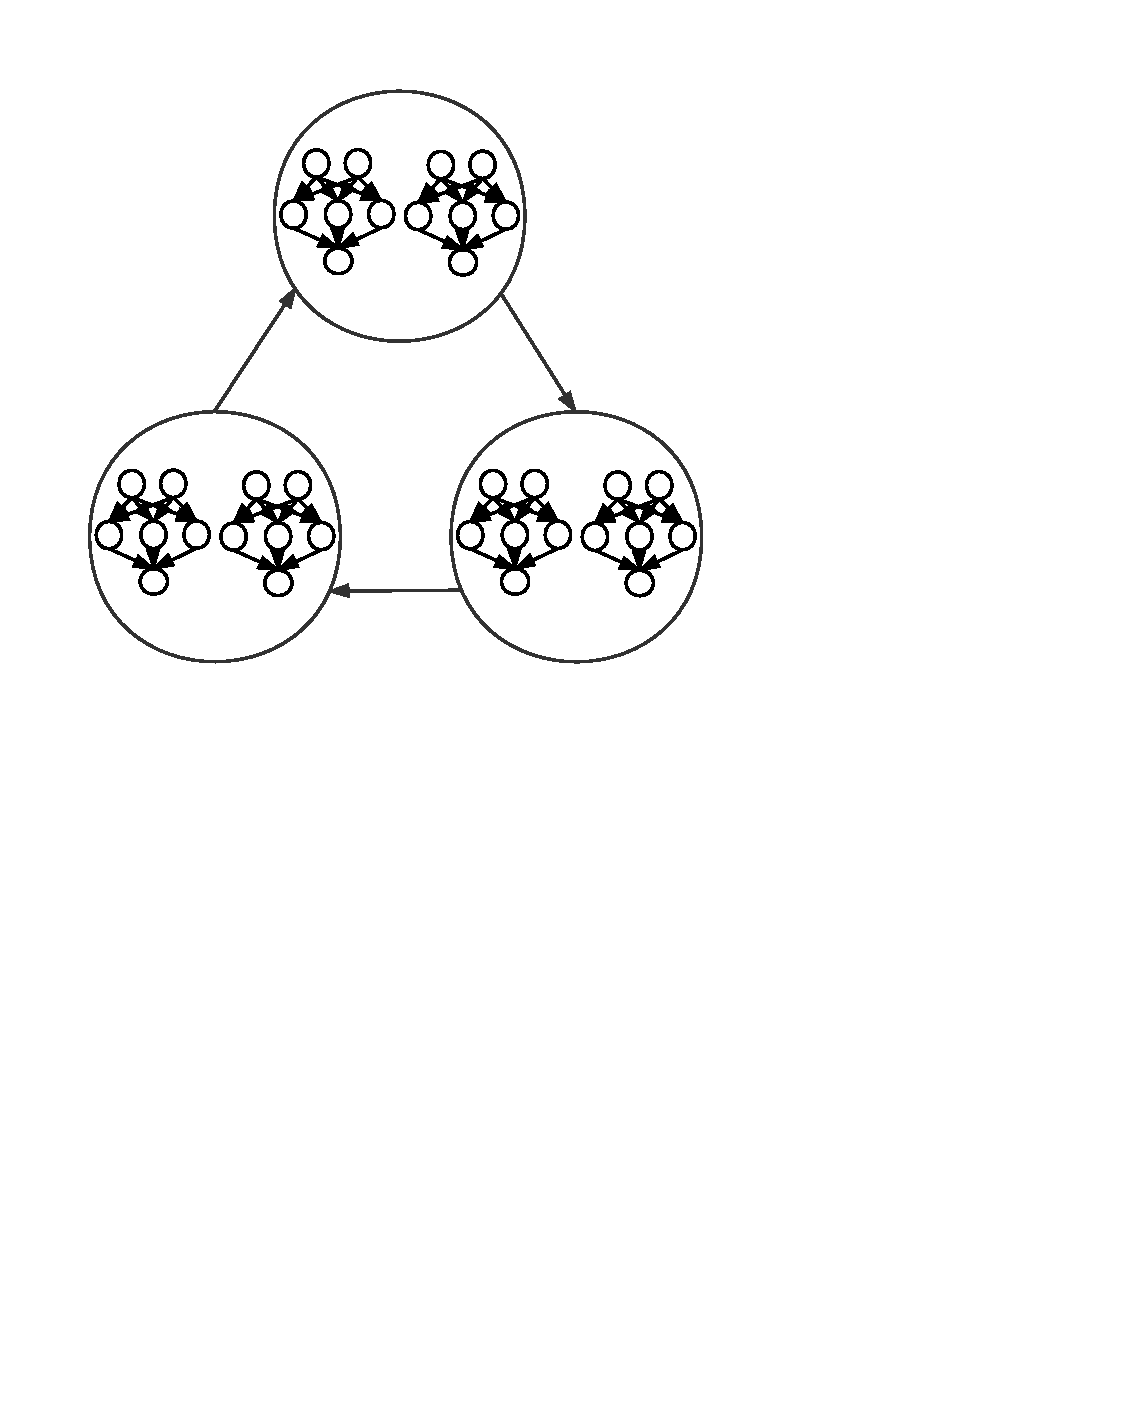
\includegraphics[width=0.6\textwidth]{Multi-DQN.pdf}
    \caption{自适应 Deep Q-Network (N=3)}
\end{figure}

如上图所示(图中 $N=3$),通过为每位选手分配一对 Deep Q-Network 之后,依次进行模拟博弈训练,基于训练数据执行 Deep Q-Learning 算法,通过前面的证明可知,这样的算法能够收敛得到 $Q(s,a)$ 函数的无偏估计值,便可基于估计函数 $\widehat{Q}(s,a)$ 推出最优策略 $\pi$ 。由于算法能够自适应地根据玩家数量调整网络参数,且每个玩家学习模型下的双神经网络能够自适应地准确消除各自的偏差,故称这样的算法为{\jiacu 自适应 Deep Q-Learning 算法}。